\documentclass[a4paper,10pt,fleqn]{article}

\usepackage{src/common/layout}

\newboolean{STANDALONE}
\setboolean{STANDALONE}{false}

\newboolean{EMBED}
\setboolean{EMBED}{false}

\setcounter{tocdepth}{4}   %= Aufnahme in das Inhaltsverzeichnis *
\setcounter{secnumdepth}{4}  % = Nummerierung vertiefen *

\setboolean{EMBED}{true}

\title{Dokumentation BLDC}
\newcommand{\EtPath}{src/BLDC}
\newcommand{\DasAndereTeam}{T27 }
\newcommand{\BLDCTeams}{T27 und T32}
\newcommand{\BLDCcollab}{Dieses Kapitel ist eine Zusammenarbeit der Gruppen \BLDCTeams. }

\begin{document}

\maketitle
\clearpage
\tableofcontents
\clearpage

\ifSTANDALONE
\section{Hardware}
\fi
\ifEMBED
\subsection{Hardware}
\fi
Die Elektrotechnik-Studierenden aus mehreren Gruppen haben sich
zusammengeschlossen um gemeinsame Probleme anzugehen. Dabei handelt es sich
um die benötigte Hard- und Software, um Motoren anzusteuern
und gegebenenfalls zu regeln. In diesem Zusammenschluss wurden drei Gruppen
gebildet, um Lösungen für DC-, Stepper- und Brushless-Motoren auszuarbeiten.
Die Idee besteht darin, dass nicht jede Gruppe für dasselbe Problem wo
möglich denselben Lösungsansatz verfolgt, sondern die Ressourcen kombiniert,
Synergien nutzt um eine bessere Lösung zu erarbeiten. Auf diese Weise kann
das Team übergreifende Arbeiten im Rahmen der PREN erlernt und
geübt werden. Somit wird Idee der Interdisziplinarität im erweiterten Sinn
Rechnung getragen. Die Gruppen und deren Mitglieder sind in der Tabelle 
\ref{tab:pren-et-overview} aufgeführt.
\begin{table}[h!]
	\centering
	\begin{tabular}{l l}
		Projekt		& Team \\
		\hline
		DC Motoren	& 39 \\
		Schrittmotor	& 27, 38 \\
		BLDC Motor	& 27, 32 \\
	\end{tabular}
	\caption{Übersicht der PREN-ET Projektgruppen}
	\label{tab:pren-et-overview}
\end{table}

\newpage
\ifSTANDALONE
\section{Brushless Motoransteuerung}
\fi
\ifEMBED
\subsection{Brushless Motoransteuerung}
\fi

\ifEMBED
    % Dieses Kapitel ist eine Zusammenarbeit der Gruppen \BLDCTeams. 
    \BLDCcollab
\fi
    \ifSTANDALONE
    \subsection{Theorie der Ansteuerung}
    \fi
    \ifEMBED
    \subsubsection{Theorie der Ansteuerung}
    \fi
    \ifEMBED
        \begin{wrapfigure}{r}{0.50\textwidth}
           	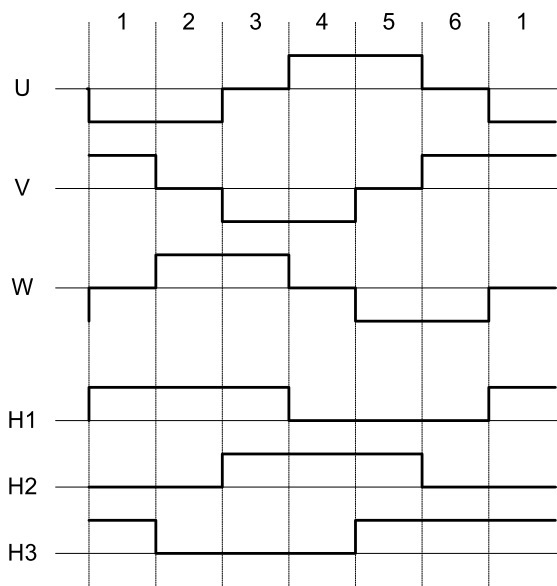
\includegraphics[scale=0.45]{\EtPath/Bilder/ZeitlicheHallSensorAnsteuerung.jpg}
           	\caption[Zeitliche Darstellung der Ansteuerung mit Hall-Sensoren]
           	{Zeitliche Darstellung der Ansteuerung mit Hall-Sensoren \cite{AppNote:BrushlessuC}}
           	\centering
            \label{abb:ZeitlicheAnsteuerungBrushlessMotor}
        \end{wrapfigure}
    \fi
        Brushless-Motoren (BLDC-Motoren) sind Synchron-Drehstrom-Motoren. Das bedeutet, sie
        werden mittels eines kontinuierlichen magnetischen Drehfeldes in Bewegung gesetzt.
        Dabei ist darauf zu achten, dass der Läufer dem Drehfeld synchron folgen kann,
        daher auch die Namensbezeichnung des Motors. Falls der Läufer dem Drehfeld nicht
        folgen kann, wird keine Spannung vom Rotor in die Statorwicklungen induziert, die
        der Erregerspannung entgegenwirkt. Daraus folgt, dass ein immenser Strom fliesst, 
        der nur von der Wicklungsimpedanz des Motors begrenzt wird.\\
        \ifSTANDALONE
           \begin{figure}[h!]
               \centering
               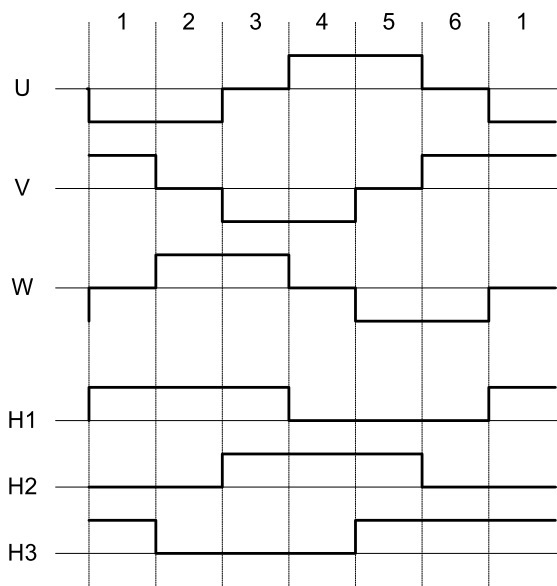
\includegraphics[scale=0.45]{\EtPath/Bilder/ZeitlicheHallSensorAnsteuerung.jpg}
               \caption[Zeitliche Darstellung der Ansteuerung mit 
                   Hall-Sensoren]{Zeitliche Darstellung der Ansteuerung mit 
                   Hall-Sensoren \cite{AppNote:BrushlessuC}}
              	\centering
               \label{abb:ZeitlicheAnsteuerungBrushlessMotor}
           \end{figure}
      \fi
       \\
        Es gibt hauptsächlich drei Methoden das Drehfeld zu generieren und zu 
        regeln. Die einfachste Methode ist die Zwangskommutierung: 
        Dabei wird ein Drehfeld erzeugt und dem Motor aufgezwungen. Der Läufer 
        muss dem Drehfeld folgen, der maximal zulässige Winkel von 90$^\circ$
        zwischen dem Feld und dem Läufer muss eingehalten werden. Wird dieser 
        Winkel überschritten, kommt der Motor zum Stillstand.\\
        \\
        Die zweite Methode zur Regelung des Motors verwendet drei Hallsensoren, die im 
        Motor integriert sind. Dies macht den Motor aufwändiger und 
        dementsprechend teurer. Die Regelung mit Hallsensoren ist 
        verhältnismässig einfach, da nach den Signalen die einzelnen Spulen 
        direkt angesteuert werden können. Der Zusammenhang zwischen der 
        Ansteuerung und den Hallsensor-Signalen ist in Abbildung 
        \ref{abb:ZeitlicheAnsteuerungBrushlessMotor} ersichtlich. Dabei stehen 
        $U$, $V$ und $W$ für die Phasenströme und $H_1$, $H_2$ und $H_3$ für die 
        entsprechenden Signale der Hallsensoren. Dieser Darstellung ist zu 
        entnehmen, wenn ein Hallsensor eine Änderung anzeigt, 
        ein Nulldurchgang im entsprechenden Stromverlauf stattgefunden hat. 
        Dies ist der Zeitpunkt, zu dem die Kommutierung durchgeführt werden 
        muss.\\
        \\
        Für die dritte Möglichkeit bildet man einen virtuellen Sternpunkt 
        und detektiert mit Komparatoren die Sternpunktdurchgänge. 
        In der Controller-Logik muss der Zeitunterschied der Kommutierung 
        bis zum durchschreiten des Sternpunktes gemessen werden. Diese Zeit 
        muss noch einmal abgewartet werden, bevor die Kommutierung durchgeführt 
        wird.
    \ifSTANDALONE
    \subsection{Neuer Ansatz}
    \fi
    \ifEMBED
    \subsubsection{Neuer Ansatz}
    \fi

        \ifEMBED
        \begin{wrapfigure}{r}{0.40\textwidth}
            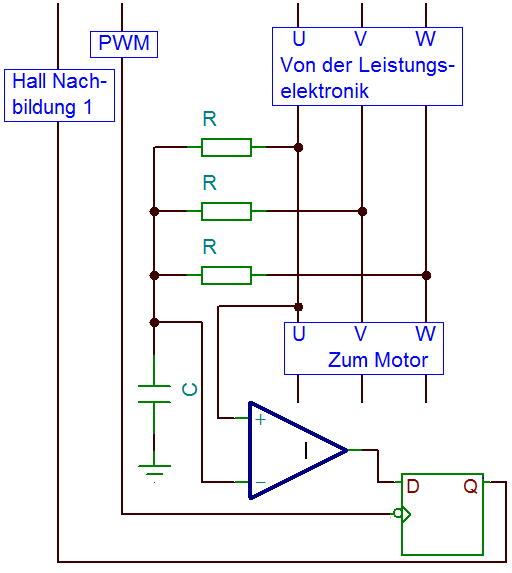
\includegraphics[scale=0.46]{\EtPath/Bilder/PrinzipDerRekonstruktion.png}
            \centering
            \caption[Schema des Rekonstruktionsprinzip]{Schema des Rekonstruktionsprinzip \cite{HSLU:Pluess}}
            \label{abb:PrinzipRekonstruktion}
            \end{wrapfigure}
        \fi
        In einem modifizierten Ansatz wird versucht, die Hallsensor-Signale 
        aus den Ansteuerungen des Motors zu gewinnen. Hierzu wird 
        eine Schaltung pro Phase benötigt, um die Nulldurchgänge beim 
        virtuellen Sternpunkt detektieren zu können. Die Abbildung 
        \ref{abb:PrinzipRekonstruktion} zeigt die Schaltung, mit der dieser Ansatz 
        realisiert werden kann. 
        \ifSTANDALONE
	\begin{figure}[h!]
            \centering
            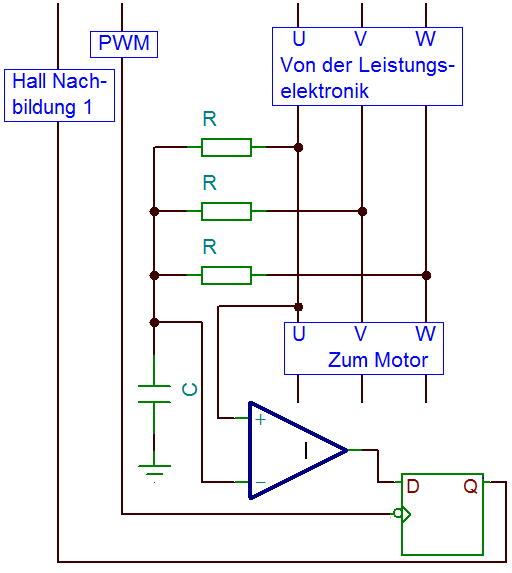
\includegraphics[scale=0.46]{\EtPath/Bilder/PrinzipDerRekonstruktion.png}
           	\caption{Schema des Rekonstruktionsprinzip \protect\cite{HSLU:Pluess}}
            \label{abb:PrinzipRekonstruktion}
        \end{figure}
        \fi
        Mit dem Flip-Flop aus Abbildung \ref{abb:PrinzipRekonstruktion} kann die PWM aus dem 
        Sensorsignal unterdrückt werden. Diese rekonstruierten 
        Hallsensor-Signale können direkt logisch verknüpft und genutzt 
        werden, um den Motor mit einer Dreiphasen-H-Brücke anzusteuern 
        \cite{HSLU:Pluess}. Anhand des zeitlichen Verlaufs, der aus Abbildung 
        \ref{abb:ZeitlicheAnsteuerungBrushlessMotor} zu entnehmen ist und der 
        Ansteuerung einer H-Brücke, ergibt sich die Wahrheitstabelle, die in 
        Abbildung \ref{abb:WahrheitstabelleAnsteuerung} ersichtlich ist. Das 
        Signal $U_h$ symbolisiert den Highside-Transistor der Phase U auf der 
        H-Brücke und die Spalte $U_l$ entspricht dem Lowside-Transistor.\\      
        
        \begin{figure}[h!]
            \begin{tabular}{ccc||cc|cc|cc||c}
                 $H_1$ & $H_2$ & $H_3$ & $U_h$ & $U_l$ & $V_h$ & $V_l$ & $W_h$ & $W_l$ & Illegal\\
            \hline 0   &   0   &   0   &   0   &   0   &   0   &   0   &   0   &   0   &   1\\
                   0   &   0   &   1   &   0   &   0   &   0   &   1   &   1   &   0   &   0\\
                   0   &   1   &   0   &   0   &   1   &   1   &   0   &   0   &   0   &   0\\
                   0   &   1   &   1   &   0   &   1   &   0   &   0   &   1   &   0   &   0\\
                   1   &   0   &   0   &   1   &   0   &   0   &   0   &   0   &   1   &   0\\
                   1   &   0   &   1   &   1   &   0   &   0   &   1   &   0   &   0   &   0\\
                   1   &   1   &   0   &   0   &   0   &   1   &   0   &   0   &   1   &   0\\
                   1   &   1   &   1   &   0   &   0   &   0   &   0   &   0   &   0   &   1\\
            \end{tabular}
           	\centering
           	\caption{Wahrheitstabelle der Ansteuerung} 
            \label{abb:WahrheitstabelleAnsteuerung}
        \end{figure}
        \parindent 0pt Die Tabelle in Abbildung 
        \ref{abb:WahrheitstabelleAnsteuerung} kann pro Signal zu folgenden 
        logischen Verknüpfung vereinfacht werden\\
        \\
        \ifSTANDALONE
        \begin{table}
            \centering
            \begin{tabular}{ccc}
                $U_h = H_1 \wedge \bar{H_2}$ & $V_h = H_2 \wedge \bar{H_3}$ & $W_h = \bar{H_1} \wedge H_3$\\
                $U_l = \bar{H_1} \wedge H_2$ & $V_l = \bar{H_2} \wedge H_3$ & $W_l = H_1 \wedge \bar{H_3}$
            \end{tabular}
        \end{table}
        \fi
        \ifEMBED
        \begin{tabular}{ccc}
            $U_h = H_1 \wedge \bar{H_2}$ & $V_h = H_2 \wedge \bar{H_3}$ & $W_h = \bar{H_1} \wedge H_3$\\
            $U_l = \bar{H_1} \wedge H_2$ & $V_l = \bar{H_2} \wedge H_3$ & $W_l = H_1 \wedge \bar{H_3}$
        \end{tabular}
        \fi

\newpage
\ifSTANDALONE
\section{Prinziptest}
\fi
\ifEMBED
\subsubsection{Aufbaubeschreibung}
    \BLDCcollab
\fi
\ifEMBED
    \begin{wrapfigure}{r}{0.55\textwidth}
       	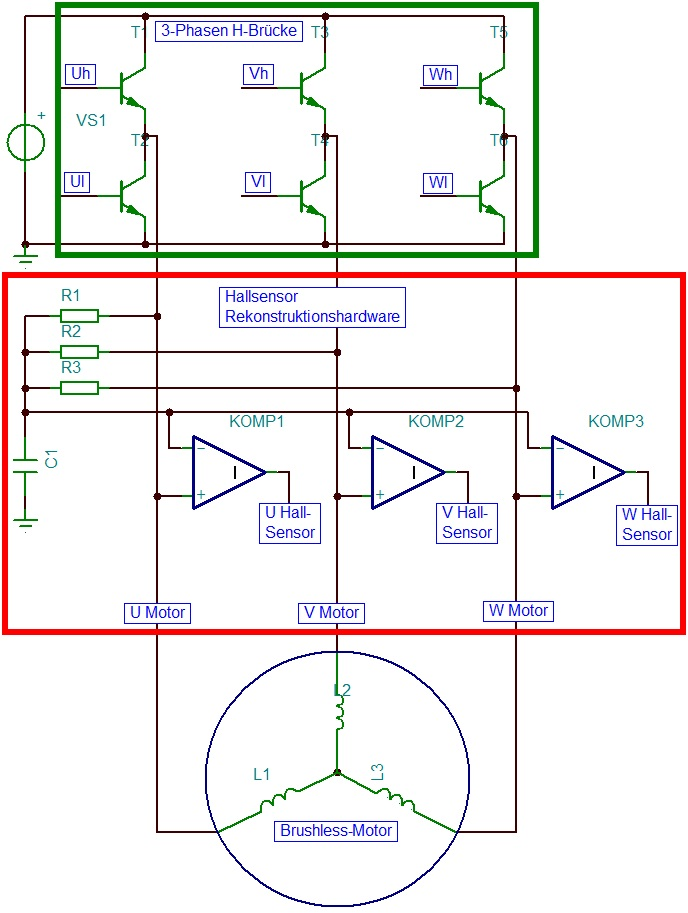
\includegraphics[scale=0.4]{\EtPath/Bilder/MotoransteuerungSchema.jpg}
       	\centering
       	\caption{Schema des Brushless-Versuchsaufbaus}
        \label{abb:MotoransteuerungSchema}
    \end{wrapfigure}
\fi
    Das Schema des Gesamtaufbaus des Tests ist in der Abbildung 
    \ref{abb:MotoransteuerungSchema} ersichtlich. Die 3-Phasen H-Brücke 
    im oberen grünen Rechteck wird direkt vom FPGA angesteuert. Die Hardware 
    dieser Brücke ermöglicht eine voll galvanisch getrennte Ansteuerung 
    mit 3.3V Logikpegeln. Diese Brücke wurde zur Verfügung gestellt und direkt
    implementiert. Die Rekonstruktion der Hallsensoren-Signale findet im rot 
    markierten Teil des Aufbaus statt. Dieser Part wurde auf einer 
    Laborplatte aufgebaut und gelötet. Die so generierten Signale 
    $U_{Hallsensor}$, $V_{Hallsensor}$, $W_{Hallsensor}$ werden einem FPGA 
    geliefert. Anhand dieser Signale steuert das FPGA die 
    H-Brücken-Transistoren mit den Signalen $U_h$, $U_l$, $V_h$, $V_l$, 
    $W_h$, $W_l$. Die im FPGA enthaltene Konfiguration besteht aus simplen 
    AND-Verknüpfungen, die die anliegenden Signale sehr schnell und 
    effizient verarbeiten können. Auf diese Weise ist es möglich, den Motor sehr 
    schnell anzusteuern.
    \ifSTANDALONE
    \begin{figure}[h!]
    	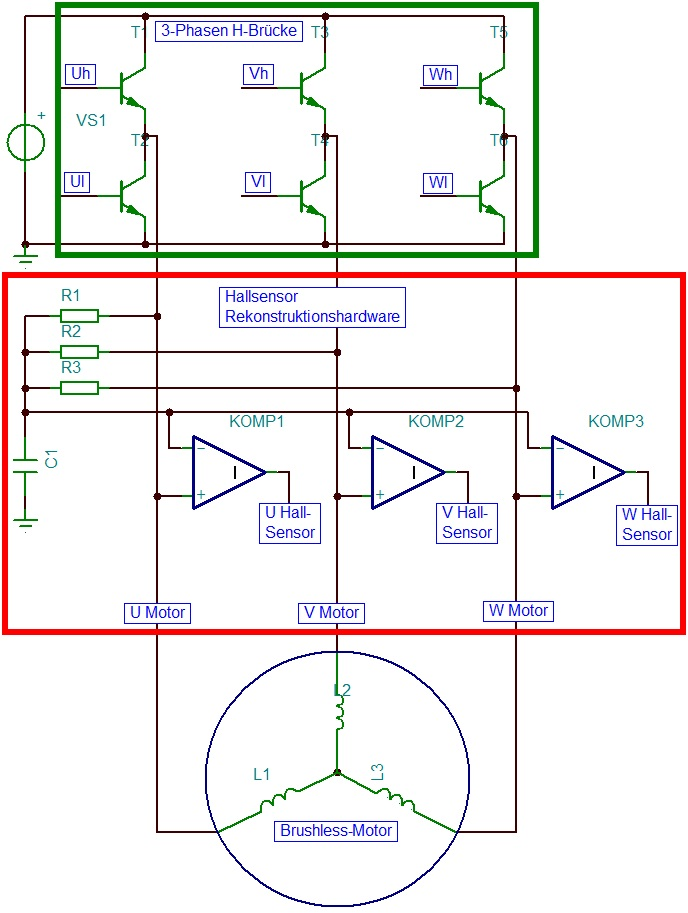
\includegraphics[scale=0.4]{\EtPath/Bilder/MotoransteuerungSchema.jpg}
       	\centering
       	\caption{Schema des Brushless-Versuchsaufbaus}
        \label{abb:MotoransteuerungSchema}
    \end{figure}
    \fi
    In der Abbildung \ref{abb:MessplatzAufbau} ist der gesamte Aufbau 
    abgebildet. Man beachte die markierten Felder. Am linken unteren Rand 
    ist der Motor befestigt. In der Mitte des Bildes ist die Hardware zur Rekonstruktion der Hallsensoren-Signale.
    Die generierten Signale werden dem FPGA in der unteren linken Ecke zugeführt. Diese 
    Signale werden logisch verknüpft und danach die sechs Signale 
    generiert, um die H-Brücke in der rechten oberen Hälfte anzusteuern. 
    Die H-Brücken wiederum treiben den Motor an.
    \begin{figure}[h!]
    %\vspace{-16pt}
       	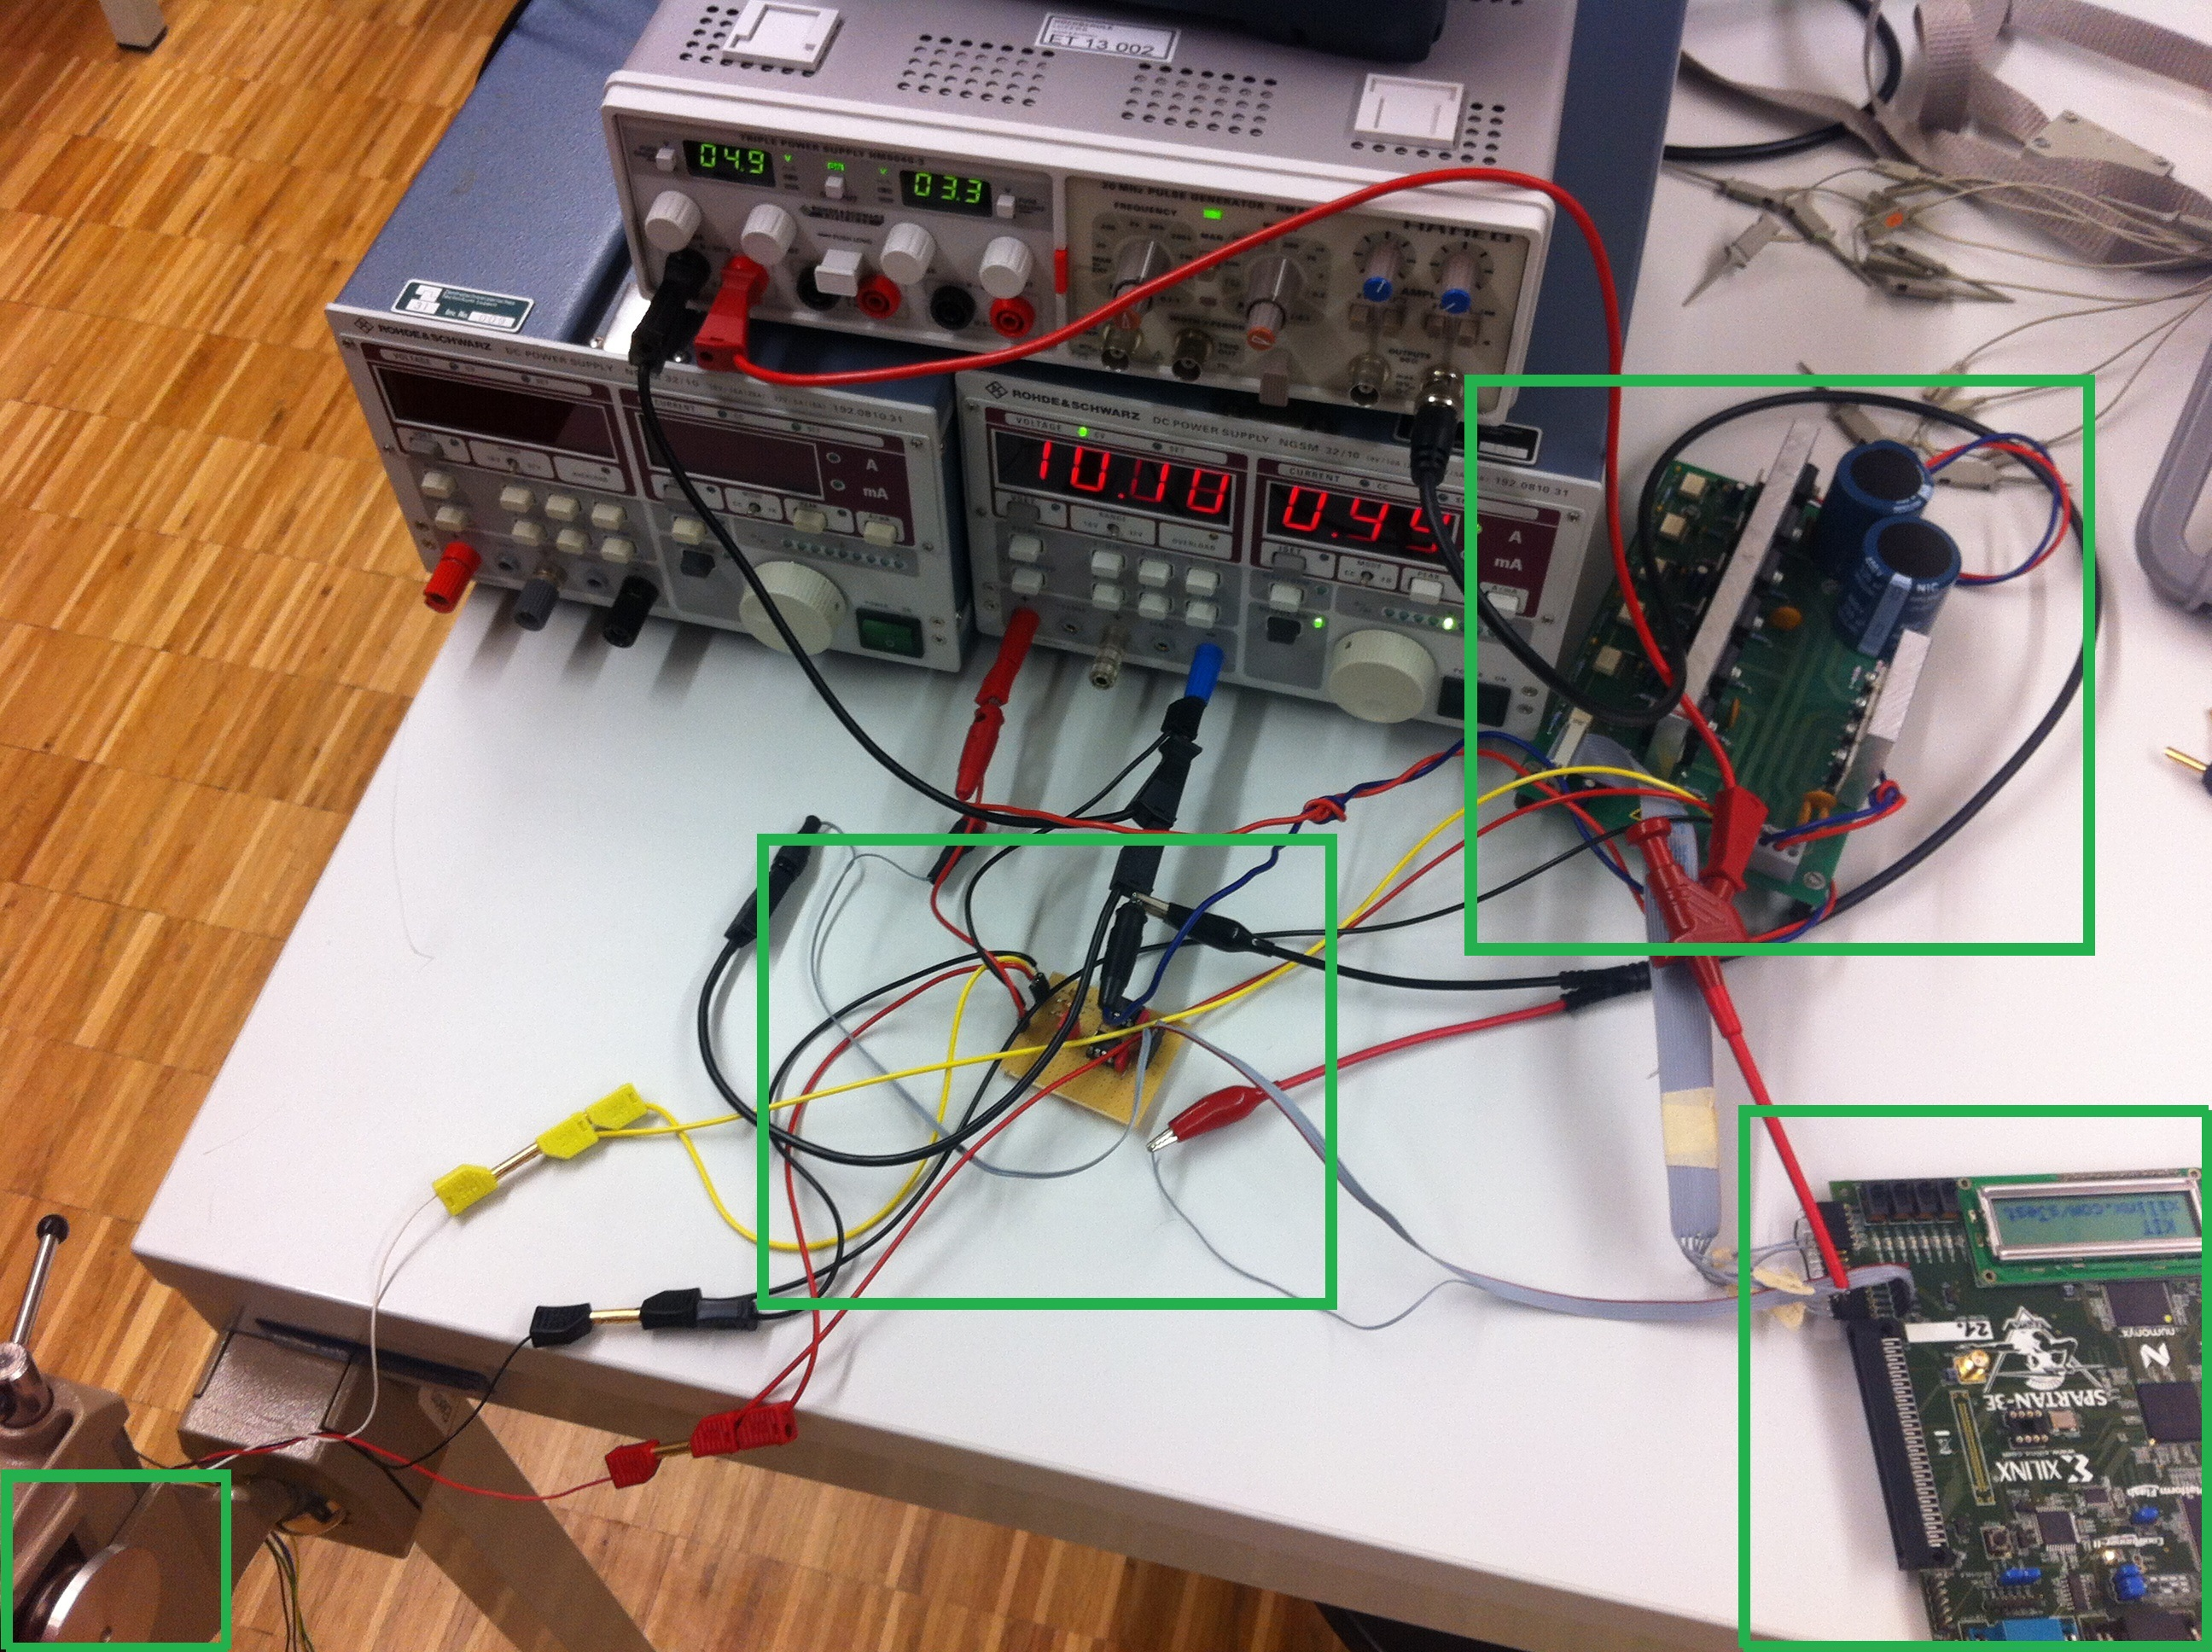
\includegraphics[scale=0.14]{\EtPath/Bilder/MessplatzAufbau.jpg}
       	\centering
       	\caption{Testaufbau} 
        \label{abb:MessplatzAufbau}
    %\vspace{-10pt}
    \end{figure}
    Die im FPGA enthaltene Logik basiert auf der Wahrheitstabelle, die in 
    Abbildung \ref{abb:WahrheitstabelleAnsteuerung} abgebildet ist.

\ifSTANDALONE
\subsection{Messmittel}
\fi
\ifEMBED
\subsubsection{Messmittel}
\fi
    \begin{table}[h!]
        \centering
        \begin{zebratabular}{lll}
            \rowcolor{gray}
            Gerät &
                Typ &
                Nummer \\
            Speisegerät & 
                Rohde \& Schwarz NGSM 32/10 &
                Inv.-Nr. 009 \\
            Oszilloskop &
                Agilent MSO6052A &
                Inv.-Nr. 44; S/N: MY44001903 \\
            Mainframe &
                Hameg HM8001-2 &
                SN: 059520046 \\
            Speisegerät &
                Hameg HM8040-3 &
                SN: 015405014 \\
            Pulsgenerator &
                Hameg HM8035 &
                Inv.-Nr. 44 \\
        \end{zebratabular}
        \caption{Messmittel des Versuchsaufbaus}
    \end{table}

\newpage
\ifSTANDALONE
\section{Fallback}
\fi
\ifEMBED
\subsection{Fallback}
\fi
Ist der Einsatz des vorgesehenen BLDC-Treibers nicht möglich, so muss eine
alternative Ansteuerung erfolgen. Eine solche kann mit einer handelsüblichen
Steuerungen aus dem Modellbau erfolgen. Eine solche BLDC-Steuerung ist per
PWM angesteuert, wobei die im Modellbau üblichen Signale gelten, wie in der
Abbildung \ref{fig:rc-pwm} dargestellt.

\begin{figure}[h!]
	\centering
	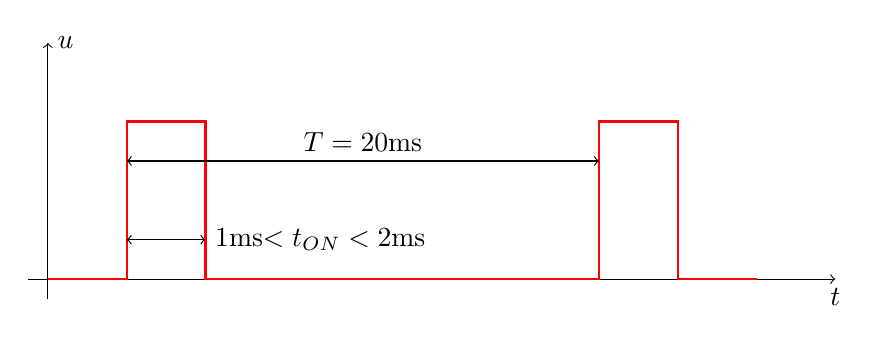
\begin{tikzpicture}
		% Achsen
		\draw[->] (-0.25,0) -- (10,0) node[anchor=north] {$t$};
		\draw[->] (0,-0.25) -- (0,3) node[anchor=west] {$u$};
		% Signal
		\draw[-,red,thick] (0,0) -- (1,0) -- (1,2) -- (2,2) -- 
			(2,0) -- (7,0) -- (7,2) -- (8,2) -- (8,0) -- (9,0);
		% Zeiten
		\draw[<->] (1,1.5) -- (7,1.5) node[midway, above] {$T=20$ms};
		\draw[<->] (1,0.5) -- (2,0.5) node[right] {$1$ms$<t_{ON}<2$ms};
	\end{tikzpicture}
	\caption{Signalverlauf eines typischen Modellbau-PWM Signals}
	\label{fig:rc-pwm}
\end{figure}

Der Einsatz von Modellbausteuerungen für BLDC-Motoren erfordert ein
Feedback der Drehzahl, da diese lediglich eine Steuerung darstellen. Die
Drehzahlregelung muss über eine externe Einheit erfolgen, beispielsweise einen
Mikrocontroller. Solche BLDC-Steuerungen werden im Modellbau typischerweise als
\emph{Regler} vertrieben und sind auch für hohe Leistungen durchaus preiswert.

\ifSTANDALONE
\subsection{Konzeptbeschreibung}
\fi
\ifEMBED
\subsubsection{Konzeptbeschreibung}
\fi
Um eine Regelung der Drehzahl des BLDC-Motors zu ermöglichen, bedarf es eines
Feebacks, welches die Drehzahl wiedergibt. Dies ist mit einem
Hall-Effekt-Schalter zu realisieren. Dieser reagiert auf die Magnetfelder,
welche durch Magnete auf dem Rotationskörper gegeben sind. Aus solch einem
Aufbau resultiert ein Feedback, welches mit Impulsen einen Segmentdurchlauf
des Rotationskörpers wiedergibt, wie in Abbildung \ref{fig:fallback-sketch}
dargestellt.
\begin{figure}[h!]
	\centering
	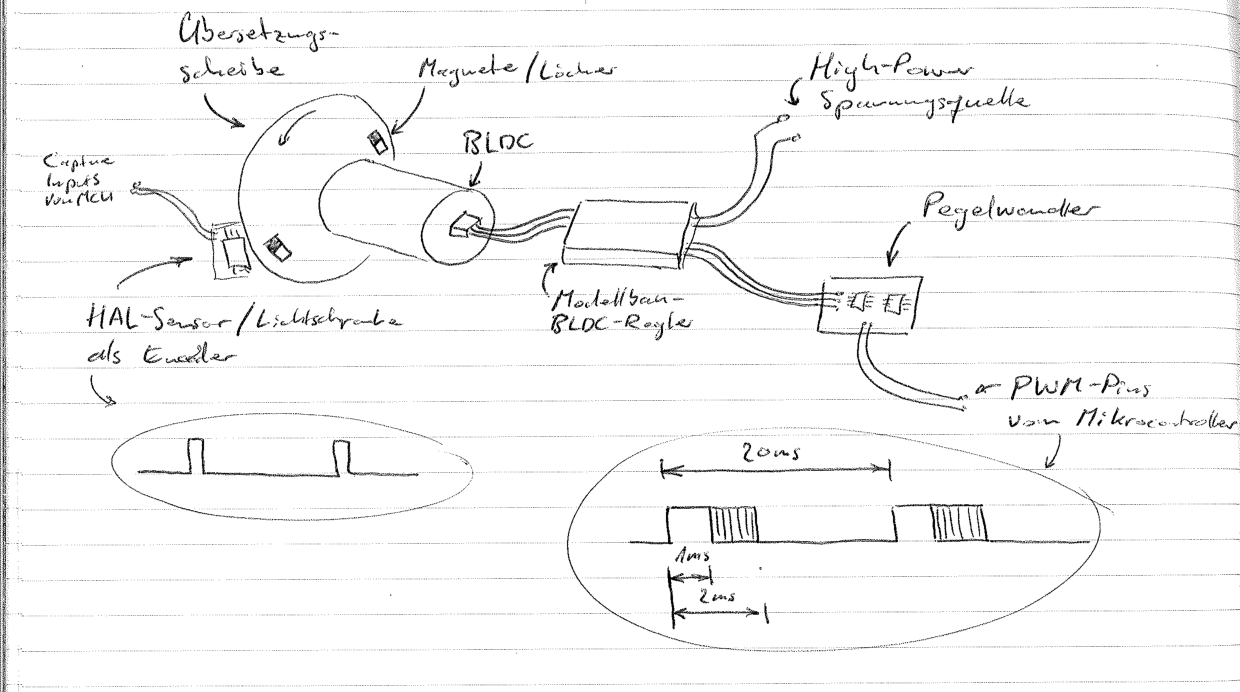
\includegraphics[width=0.8\textwidth]{\EtPath/Bilder/fallback_sketch_1.pdf}
	\caption{Erste Skizze des Fallback-Konzepts}
	\label{fig:fallback-sketch}
\end{figure}
Dieses Feedback wird mittels eines Mikrocontrollers ausgewertet und regelt
damit den Input der Steuerung mit dem PWM-Signal beziehungsweise der Impulsdauer.
Das Einlesen einer Flanke, die Zeitmessung bis zur nächsten Flanke und die
Stellung eines PWM-Signals, sind Tasks welche übliche Mikrocontroller direkt
durch ihre Peripherie-Module ausführen können. Dies ermöglicht eine einfache
Adaption in ein bestehendes Modell, denn es werden lediglich zwei Timer-IO
für diesen Fallback verwendet. Je nach Mikrocontroller ist ein Pegelwandler
für die PWM-Signale notwendig.

\newpage
\ifSTANDALONE
\section{Encoder \& Drehzahlgeber}
\fi
\ifEMBED
\subsubsection{Encoder \& Drehzahlgeber}
\fi

Die vorgesehenen Motorfunktionen verlangen lediglich beim Brushlessmotor
nach einem Feedback über die Rotation des Motors, da der Schrittmotor
definiert und fein granuliert betrieben wird. Der Gleichstrommotor stellt
keinerlei Ansprüche, weder an die Drehzahl, noch an die Position.

Encoder sind relativ teuer und der Einsatz des Brushlessmotors verlangt
lediglich nach einem Feedback zur Rotation beziehungsweise Winkelgeschwindigkeit.
Die absolute oder relative Position ist für die Anwendung nicht von
Bedeutung. Somit lässt sich ein einfaches Feedback vorsehen, für die
Regelung der Drehzahl mit optischen oder magnetischen Elementen.
\ifSTANDALONE
\begin{figure}[h!]
	\centering
	\begin{tikzpicture}
		% Koordinaten
		\draw[->] (-0.5, 0) -- (8, 0) node[anchor=north] {$t$};
		\draw[->] (0, -1.5) -- (0, 3) node[anchor=east] {$u,\varphi$};
		% Rotation
		\draw[blue] (0,0) sin (1,1) cos (2,0) sin (3,-1) cos (4,0)
			sin (5,1) cos (6,0) sin (7,-1)
			node[right] {$\varphi$};
		% Signal
		\draw[-, thick, red]
			(0,0) -- (0.8,0) -- (0.8,2) -- (1.2,2) -- (1.2,0) -- 
			(4.8,0) -- (4.8,2) -- (5.2,2) -- (5.2,0) -- (7.5,0);
		% Messung
		\draw[<->] (0.8,1.5) -- (4.8,1.5) node[midway, above] {$t_{r}$};
	\end{tikzpicture}
	\caption{Vereinfachtes Puls-Feedback eines Hall-Effekt-Schalters}
	\label{fig:hall-effekt-schalter}
\end{figure}
\fi
\ifEMBED
\begin{figure}[h!]
	\centering
	\begin{tikzpicture}
		% Koordinaten
		\draw[->] (-0.5, 0) -- (8, 0) node[anchor=north] {$t$};
		\draw[->] (0, -1.5) -- (0, 3) node[anchor=east] {$u,\varphi$};
		% Rotation
		\draw[blue] (0,0) sin (1,1) cos (2,0) sin (3,-1) cos (4,0)
			sin (5,1) cos (6,0) sin (7,-1)
			node[right] {$\varphi$};
		% Signal
		\draw[-, thick, red]
			(0,0) -- (0.8,0) -- (0.8,2) -- (1.2,2) -- (1.2,0) -- 
			(4.8,0) -- (4.8,2) -- (5.2,2) -- (5.2,0) -- (7.5,0);
		% Messung
		\draw[<->] (0.8,1.5) -- (4.8,1.5) node[midway, above] {$t_{r}$};
	\end{tikzpicture}
	\caption{Vereinfachtes Puls-Feedback eines Hall-Effekt-Schalters}
	\label{fig:hall-effekt-schalter}
\end{figure}
\fi
Als optisches Messinstrument kann eine Lichtschranke mit 
Reflexionsstreifen oder Löchern eingesetzt werden. Diese verlangen
nur nach einer geringfügigen Modifikation des rotierenden Körpers und
sind relativ günstig. Optische Messtechnik hat den Nachteil, das
Störungen relativ leicht in die Messung einfliessen können, was fatale
Folgen für die Regelung hat. Magnetische Messinstrumente sind gegenüber
Störungen deutlich resistenter, da hierfür starke Magnetfelder benötigt
werden, welche so nicht einfach auftreten. Der Einsatz einer solchen Messtechnik
verlangt jedoch nach einer Modifikation der Mechanik, da Magnete in den
rotierenden Körper eingebaut werden müssen. Dies birgt ein gewisses
Risiko für mechanische Unwucht des Rotationskörpers.

\ifSTANDALONE
\subsection{Magnetischer Drehzahlgeber}
\fi
\ifEMBED
\newpage
\paragraph{Magnetischer Drehzahlgeber}$~~$\vspace{2mm}\\
\fi
Um einen eigenen magnetischen Drehzahlgeber zu erstellen wird ein
sogenannter Hall-Effekt-Schalter eingesetzt. Dieser reagiert mit seinem Ausgang
auf ein auftretendes Magnetfeld. Das Gegenstück zum Hall-Effekt-Schalter
ist ein Magnet, welcher in das rotierende Objekt eingebaut wird. Aus 
mechanischen Gründen, wie etwa der Unwucht, werden typischerweise 2 Magnete
oder ein Vielfaches davon in den rotierenden Körper eingebaut.

Bei der Rotation des Körpers entstehen durch das Passieren der Magnete
am Hall-Effekt-Schalter Impulse. Aus diesen Impulsen lässt sich mit einer
Zeitmessung direkt die Drehzahl bestimmen. Die Abbildung 
\ref{fig:hall-effekt-schalter} illustriert das Prinzip anhand eines
Beispiels mit einem Magneten am Rotationskörper.
%
\ifSTANDALONE
\begin{figure}[h!]
	\centering
	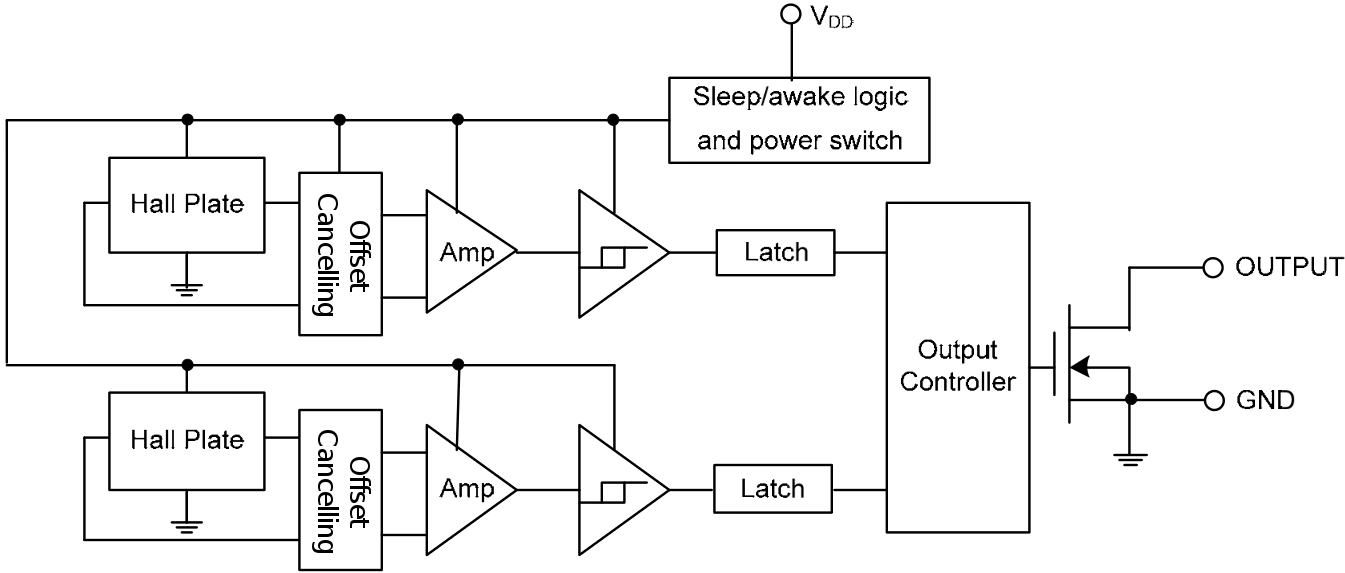
\includegraphics[width=0.75\textwidth]{\EtPath/Bilder/AH180N_functional.png}
	\caption{Funktionelles Blockschaltbild des Hall-Effekt-Schalters AH180N}
	\label{fig:AH180N_functional}
\end{figure}
\fi
%
\ifEMBED
\begin{figure}[h!]
	\centering
	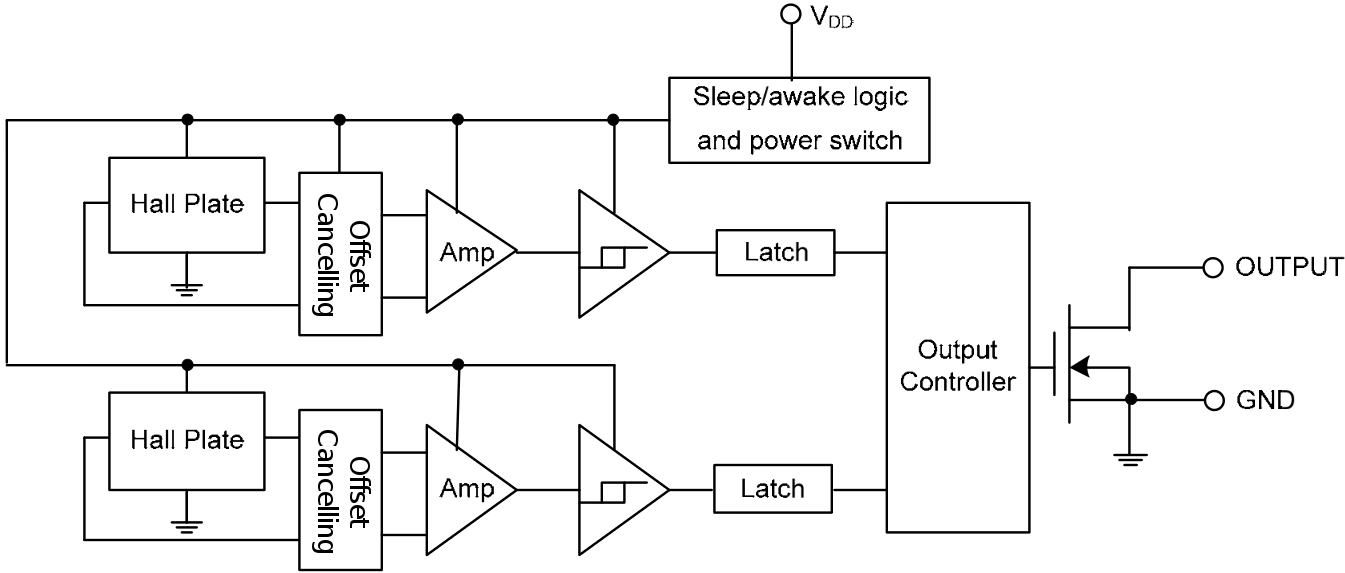
\includegraphics[width=0.75\textwidth]{\EtPath/Bilder/AH180N_functional.png}
	\caption{Funktionelles Blockschaltbild des Hall-Effekt-Schalters AH180N}
	\label{fig:AH180N_functional}
\end{figure}
\fi
%
Ein solches Verfahren lohnt sich bei schnellen Winkelgeschwindigkeiten
und ist für diesen Anwendungsfall sehr effizient. Zugehörige
Hall-Effekt-Schalter lassen sich einfach montieren und sind gegen Störungen
sehr robust. Ein mögliches Modell für einen Hall-Effekt-Schalter ist der
AH180N. Dieser bietet einen Open-Drain Ausgang, welcher somit logische Pegel
liefert (siehe Abbildung \ref{fig:AH180N_functional}). Interessant ist diese
Art von Drehzahl-Geber insbesondere durch ihren geringen Preis, denn solche
Hall-Effekt-Schalter, wie der AH180N, befinden sich im Preissegment von 
unter einem Franken.
\clearpage

\begin{flushleft}
    \renewcommand{\refname}{Literatur- und Quellenverzeichnis}
%        \{\refname}{Quellenverzeichnis}
    \bibliography{src/common/ET-Gruppe_Source}{} %!!! Kein Leerzeichen nach dem , !!!!
\end{flushleft}

\end{document}
